\documentclass[12pt]{article}
\usepackage{amsmath} 
\usepackage[round]{natbib}
\usepackage{geometry}
% \usepackage{times}
\usepackage{graphicx}
% \usepackage{courier}
\usepackage{mathpazo}
\usepackage{mathrsfs}
\usepackage{bm}
\usepackage[colorlinks,linkcolor=red,anchorcolor=blue,citecolor=blue]{hyperref}
\usepackage{amsthm}
\usepackage{ulem}
\geometry{verbose,letterpaper,tmargin=1in,bmargin=.75in,lmargin=.75in,rmargin=1in}
\usepackage{booktabs}

\title{Quantile Regression with Monotone Dropout Missingness}
\date{\today}
\author{}

\newtheorem{thm}{Theorem}[section]
\newtheorem{deff}[thm]{Definition}
\newtheorem{rmk}[thm]{Remark}
% \newtheorem{prf}[thm]{Proof}
\newtheorem{cor}[thm]{Corollary}
\newtheorem{emp}[thm]{Example}
\newtheorem{lem}[thm]{Lemma}
\newtheorem{pps}[thm]{Proposition}

\newcommand{\polya}{P\'{o}lya}
\newcommand{\iid}{\stackrel{\text{i.i.d}}{\sim}}
\DeclareMathOperator{\pr}{p}
\DeclareMathOperator{\prob}{Pr}
\DeclareMathOperator{\pt}{PT}

\begin{document}

\maketitle{}

\section{Introduction}
The structure of this article is as below: first, we introduce our
quantile regression methods to deal with monotone dropout in bivariate
normal mixed model in section \ref{sec:bi}. Then in section
\ref{sec:tri}, we generalize our method to trivariate case. Section
\ref{sec:general} describes our proposed method in generalized cases.
Computation details are presented in section
\ref{sec:computation}. And we also include a simulation study to
demonstrate the performance of our algorithm in section
\ref{sec:simulation}.

\section{Bivariate Normal Mixed Model with Monotone Dropout}
\label{sec:bi}

In this section, we first introduce the bivariate scenario with
monotone dropout, then describe our proposed quantile regression model
in section \ref{sec:model}. And we will give more details on deploying
MAR and MNAR and computation in section \ref{sec:sa} and section
\ref{sec:computation}.

Let $\bm{Y} = (Y_{1}, Y_{2})^{T}$ and $R = I\{Y_2 \text{
  observed}\}$. Suppose we are interested in the $\tau$-th
marginalized quantile regression coefficients $\bm \gamma = (\bm
\gamma^{\tau}_1, \bm \gamma^{\tau}_2)$, where
\begin{align*}
  \bm \gamma_1^{\tau} & = (\gamma_{01}^{\tau}, \gamma^{\tau}_{11}), \\
  \bm \gamma_{2}^{\tau} & = (\gamma_{02}^{\tau}, \gamma^{\tau}_{12}),
\end{align*}
such that
\begin{align}
  \label{eq:quan1}
  \pr (Y_{i1} \leq \gamma^{\tau}_{01} + x_i \gamma^{\tau}_{11} | x_i ) & = \tau ,\\
  \label{eq:quan2}
  \pr (Y_{i2} \leq \gamma^{\tau}_{02} + x_i \gamma^{\tau}_{12} | x_i )
  & = \tau .
\end{align}
Here we assume there is only one single covariate $x_i$ for each
subject $i$, which is constant across treatments or time points, while
the quantile regression coefficients $\bm \gamma^{\tau}$ are time
varying.

\subsection{Model Setting}
\label{sec:model}
To adopt mixed model to deal with missingness, we assume $\bm Y$
follows bivariate normal distribution:
\begin{align*}
  \bm{Y}|R = r &\sim \textrm{N}(\bm{\mu}^{(r)}, \Sigma^{(r)}), r = 0, 1,\\
  R & \sim \textrm{Ber}(\phi).
\end{align*}
Reparametrize the above model as
\begin{align}
  \label{eq:model1}
  Y_{i1}|R = r, x_i &\sim \textrm{N}(\Delta_{i1} + \beta_{01}^{(r)} + x_i\beta_{11}^{(r)}, \sigma_{11}^{(r)}),\\
  \label{eq:model2}
  Y_{i2}|R = r, x_i, y_{i1} & \sim \textrm{N}(\Delta_{i2} +
  \beta_{02}^{(r)} + x_i\beta_{12}^{(r)} + y_{i1}\beta_{22}^{(r)},
  \sigma_{2|1}^{(r)}).
\end{align}
where the quantity $\Delta_{it}, t = 1, 2$ is determined by other
parameters in the model and can be solved from
\begin{align}
  \label{eq:const1}
  \tau & =  \sum_{r = 0}^1 \pr (Y_{i1} \leq \gamma^{\tau}_{01} + x_i \gamma^{\tau}_{11} | x_i , R = r) \pr (R = r), \\
  \label{eq:const2}
  \tau & = \sum_{r = 0}^{1} \pr (Y_{i2} \leq \gamma^{\tau}_{02} + x_i
  \gamma^{\tau}_{12} | x_i , R = r) \pr (R = r).
\end{align}
Specific derivation can be found in section \ref{sec:computation}.

In this section we consider $\pr (R = 1|x_i) = \pr (R = 1) = \pi = 1 -
\pr (R = 0)$, which means missingness does not depend on covariates
(missingness depending on covariates could be a further topic in
future research).

Meanwhile, for identifiability issue in equation (\ref{eq:model1}) and
(\ref{eq:model2}) , we put constraints on the $\beta$ parameters:
\begin{align}
  \label{eq:beta01}
  \beta_{01}^{(1)} + \beta_{01}^{(0)} & = 0 ,\\
  \label{eq:beta11}
  \beta_{11}^{(1)} + \beta_{11}^{(0)} & = 0, \\
  \label{eq:beta02}
  \beta_{02}^{(1)} + \beta_{02}^{(0)} & = 0, \\
  \label{eq:beta12}
  \beta_{12}^{(1)} + \beta_{12}^{(0)} & = 0, \\
  \label{eq:beta22}
  \beta_{22}^{(1)} + \beta_{22}^{(0)} & = 0.
\end{align}

\subsection{Sensitivity Analysis}
\label{sec:sa}

For identifiability issue in equation (\ref{eq:model2}), we put
constraints (\ref{eq:beta02} - \ref{eq:beta22}), thus we denote
\begin{align}
  \label{eq:c0}
  \beta_{02}^{(1)} & = - \beta_{02}^{(0)} ,\\
  \label{eq:c1}
  \beta_{12}^{(1)} & = -\beta_{12}^{(0)}, \\
  \label{eq:c2}
  \beta_{22}^{(2)} & = -\beta_{22}^{(0)}, \\
  \label{eq:cs}
  \sigma_{2|1}^{(0)} & = \lambda\sigma_{2|1}^{(1)}.
\end{align}
And when $R = 0$, $Y_{i2}|R = 0$ is not observed, $\bm \xi_s =
(\beta_{02}^{(0)}, \beta_{12}^{(0)}, \beta_{22}^{(0)}, \lambda)$ could
be a group of sensitivity parameters. We illustrate how to deploy MAR
and MNAR assumption from both frequentist way and Bayesian framework.

\begin{itemize}
\item \textbf{Frequentist way: }

  When $\bm \xi_s = \bm \xi_{s0} = (0, 0, 0, 1)$, it yields
  $p(Y_{i2}|y_{i1}, x_i, R = 1) = p(Y_{i2}| y_{i1}, x_i, R = 0)$,
  where MAR condition satisfies. If $\bm \xi_s$ is fixed at $\bm \xi_s
  \neq \bm \xi_{s0}$, then $\pr (R | Y_{i1}, Y_{i2}) \neq \pr (R |
  Y_{i1})$, thus the missing mechanism is missing not at random.
\item \textbf{Bayesian Framework: }

  We put priors on $(\bm \xi_s, \bm \xi_m)$ ($\bm \xi_m$ are
  identifiable parameters) as :
  \begin{displaymath}
    p(\bm \xi_s, \bm \xi_m) = p(\bm \xi_s) p(\bm \xi_m).
  \end{displaymath}
  If we assume MAR with no uncertainty, the prior of $\bm \xi_s$ is
  $\pr(\bm \xi_s = (0, 0, 0, 1)) = 1$. Sensitivity analysis can be
  executed through putting a set of priors on $\bm \xi_s$ to check the
  effect of priors on the posterior inference about quantile
  regression coefficients $\bm \gamma_{ij}^{\tau}$. For example, if
  MAR is assumed with uncertainty, priors can be assigned as
  $\textrm{E}(\bm \xi_s) = (0, 0, 0, 1)$ with $\textrm{Var}(\bm \xi_s)
  \neq \bm 0$. If we assume MNAR with no uncertainty, we can put
  priors satisfying $\textrm{E}(\bm \xi_s) = \Delta_{\xi}$, where
  $\Delta_{\xi} \neq (0, 0, 0, 1)$ and $\textrm{Var}(\bm \xi_s) = \bm
  0$. If MNAR is assumed with uncertainty, then priors could be
  $\textrm{E}(\bm \xi_s) = \Delta_{\xi}$, where $\Delta_{\xi} \neq (0,
  0, 0, 1)$ and $\textrm{Var}(\bm \xi_s) \neq \bm 0$.
\end{itemize}

\subsection{Computation}
\label{sec:computation}
In section \ref{sec:deltacal} , we give details on how to calculate
$\Delta_{it}$ in model (\ref{eq:model1}, \ref{eq:model2}) for $t = 1,
2$ . Then we illustrate how to get maximum likelihood estimator using
gradient descent algorithm in section \ref{sec:mle}. Last, we present
the Bayesian sampling procedure in section \ref{sec:bayesian}.

\subsubsection{$\Delta$ Calculation}
\label{sec:deltacal}

First we illustrate how to calculate $\Delta_{i1}, \Delta_{i2}$ given
all the other parameters $\bm \xi = (\bm \xi_m, \xi_s)$ =
($\gamma_{01}, \gamma_{11}, \gamma_{02}, \gamma_{12}, R, x_i,
\beta_{01}^{(1)}, \beta_{11}^{(1)}, \beta_{02}^{(0)},
\beta_{12}^{(0)}, \beta_{22}^{(0)}, \sigma_{11}^{(1)},
\sigma_{11}^{(0)}, \sigma_{2|1}^{(1)}, \lambda, \phi$).

\begin{itemize}
\item \textbf{$\Delta_{i1}: $} Expand equation (\ref{eq:const1}) with
  constraints (\ref{eq:beta01}, \ref{eq:beta11}):
  \begin{align}
    \tau & = \pr (R = 1 | x_i) \pr (Y_{i1} \leq \gamma^{\tau}_{01} + x_i \gamma^{\tau}_{11} | x_i , R = 1) + \pr(R = 0 | x_i) \pr (Y_{i1} \leq \gamma^{\tau}_{01} + x_i \gamma^{\tau}_{11} | x_i , R = 0) \nonumber \\
    & = \pi F_{i1}^{(1)} (\gamma^{\tau}_{01} + x_i \gamma^{\tau}_{11};
    \Delta_{i1}, \beta_{01}^{(1)}, \beta_{11}^{(1)}, x_i,
    \sigma_{11}^{(1)}) + (1-\pi)F_{i1}^{(0)} (\gamma^{\tau}_{01} + x_i
    \gamma^{\tau}_{11};
    \Delta_{i1}, \beta_{01}^{(0)}, \beta_{11}^{(0)}, x_i, \sigma_{11}^{(0)}) , \nonumber \\
    \label{eq:solve1}
    & = \pi \Phi \left( \frac{\gamma_{01}+ x_i\gamma_{11} -
        \Delta_{i1} - \beta_{01}^{(1)} -
        x_i\beta_{11}^{(1)}}{\sigma_{11}^{(1)}} \right) + (1-\pi) \Phi
    \left( \frac{\gamma_{01} + x_i\gamma_{11} - \Delta_{i1} +
        \beta_{01}^{(1)} + x_i\beta_{11}^{(1)}}{\sigma_{11}^{(0)}}
    \right),
  \end{align}
  where $\Phi$ is the standard normal CDF. Because equation
  (\ref{eq:solve1}) is continuous and monotone on $\Delta_{i1}$, it
  can be solved by standard numerical root-find method without much
  difficulty, for example, the bisection method.

\item \textbf{$\Delta_{i2}: $} First we introduce a lemma:
  \begin{lem}
    An integral of a normal CDF over a non-standard normal
    distribution can be simplified to a closed form in terms of
    another normal CDF:
    \begin{equation}
      \label{eq:lem}
      \int \Phi \left( \frac{x-b}{a} \right) d\Phi(x; \mu, \sigma)  = 
      \begin{cases}
        1- \Phi \left( \frac{b-\mu}{\sigma} \big / \sqrt{\frac{a^2}{\sigma^2}+1} \right) & a > 0, \\
        \Phi \left( \frac{b-\mu}{\sigma} \big /
          \sqrt{\frac{a^2}{\sigma^2}+1} \right) & a < 0 ,
      \end{cases}
    \end{equation}
    where $\Phi(x; \mu, \sigma)$ stands for a CDF of normal
    distribution with mean $\mu$ and standard deviation $\sigma$.
  \end{lem}
  Proof of lemma can be seen in appendix \ref{sec:proof}.

  Hence, expand equation (\ref{eq:const2}) with constraints
  (\ref{eq:beta02} to \ref{eq:beta22}) similarly to get
  \begin{align}
    \tau & = \pr (R = 1) \pr (Y_{i2} \leq \gamma^{\tau}_{02} + x_i
    \gamma^{\tau}_{12} | x_i , R = 1) + \pr (R = 0) \pr (Y_{i2} \leq
    \gamma^{\tau}_{02} + x_i
    \gamma^{\tau}_{12} | x_i , R = 0)  \nonumber\\
    & = \pi \int \pr (y_{i2} \leq \gamma^{\tau}_{02} + x_i \gamma^{\tau}_{12} | x_i , y_{i1}, R = 1) dF_{i1}^{(1)}(y_{i1}; \Delta_{i1}, x_i, \beta_{*1}^{(1)}, \sigma_{11}^{(1)})  \nonumber\\
    & \quad + (1-\pi) \int \pr (y_{i2} \leq \gamma^{\tau}_{02} + x_i \gamma^{\tau}_{12} | x_i , y_{i1}, R = 0) dF_{i1}^{(0)}(y_{i1}; \Delta_{i1}, x_i, \beta_{*1}^{(0)}, \sigma_{11}^{(0)}) \nonumber \\
    & = \pi \int F_{i2|1}^{(1)} (\gamma^{\tau}_{02} + x_i \gamma^{\tau}_{12} ; \Delta_{i2}, \beta_{*2}^{(1)}, \sigma_{2|1}^{(1)}, x_i , y_{i1}) dF_{i1}^{(1)}(y_{i1}; \Delta_{i1}, x_i, \beta_{*1}^{(1)}, \sigma_{11}^{(1)})  \nonumber\\
    & \quad + (1-\pi) \int F_{i2|1}^{(0)} (\gamma^{\tau}_{02} + x_i \gamma^{\tau}_{12} ; \Delta_{i2},\beta_{*2}^{(0)}, \sigma_{2|1}^{(0)},  x_i , y_{i1}) dF_{i1}^{(0)}(y_{i1}; \Delta_{i1}, x_i, \beta_{*1}^{(0)}, \sigma_{11}^{(0)}), \nonumber\\
    & = \pi \int \Phi \left( \frac{\gamma_{02} + x_i\gamma_{12} - \Delta_{i2} + \beta_{02}^{(0)} + x_i\beta_{12}^{(0)} + y_{i1}\beta_{22}^{(0)}}{\sigma_{2|1}^{(1)}} \right) dF_{i1}^{(1)}(y_{i1}; \Delta_{i1}, x_i, \beta_{*1}^{(1)}, \sigma_{11}^{(1)}) \nonumber\\
    \label{eq:solve2}
    & \quad + (1-\pi) \int \Phi \left( \frac{\gamma_{02} +
        x_i\gamma_{12} - \Delta_{i2} - \beta_{02}^{(0)} -
        x_i\beta_{12}^{(0)} -
        y_{i1}\beta_{22}^{(0)}}{\lambda\sigma_{2|1}^{(1)}} \right)
    dF_{i1}^{(0)}(y_{i1}; \Delta_{i1}, x_i, \beta_{*1}^{(0)},
    \sigma_{11}^{(0)}).
  \end{align}
  By notations in (\ref{eq:c0} to \ref{eq:cs}) and lemma
  (\ref{eq:lem}), the integral on the right hand side of above
  equation (\ref{eq:solve2}) can be simplified as
  \begin{align*}
    &    \int \Phi \left( \frac{\gamma_{02} + x_i\gamma_{12} - \Delta_{i2} + \beta_{02}^{(0)} + x_i\beta_{12}^{(0)} + y_{i1}\beta_{22}^{(0)}}{\sigma_{2|1}^{(1)}} \right) dF_{i1}^{(1)}(y_{i1}; \Delta_{i1}, x_i, \beta_{*1}^{(1)}, \sigma_{11}^{(1)}) \\
    &   = \int \Phi \left( \frac{y_{i1} - (\Delta_{i2} - \gamma_{02} - x \gamma_{12} - \beta_{02}^{(0)} - x\beta_{12}^{(0)})/\beta_{22}^{(0)}}{\sigma_{2|1}/\beta_{22}^{(0)}} \right) dF_{i1}^{(1)}(y_{i1}; \Delta_{i1}+\beta_{01}^{(1)} + x\beta_{11}^{(1)}, \sigma_{11}^{(1)}) \\
    & =
    \begin{cases}
      1 - \Phi \left( \frac{(\Delta_{i2} - \gamma_{02} - x \gamma_{12} - \beta_{02}^{(0)} - x\beta_{12}^{(0)})/\beta_{22}^{(0)} - (\Delta_{i1}+\beta_{01}^{(1)} + x\beta_{11}^{(1)}) }{\sigma_{11}^{(1)}} \big / \sqrt{\frac{\sigma_{2|1}^2}{\beta_{22}^{(0)2} \sigma_{11}^{(1)2}} +1} \right) & \beta_{22}^{(0)} > 0\\
      \Phi \left( \frac{(\Delta_{i2} - \gamma_{02} - x \gamma_{12} -
          \beta_{02}^{(0)} - x\beta_{12}^{(0)})/\beta_{22}^{(0)} -
          (\Delta_{i1}+\beta_{01}^{(1)} + x\beta_{11}^{(1)})
        }{\sigma_{11}^{(1)}} \big /
        \sqrt{\frac{\sigma_{2|1}^2}{\beta_{22}^{(0)2}
            \sigma_{11}^{(1)2}} +1} \right)& \beta_{22}^{(0)} < 0
    \end{cases}
  \end{align*}

  and

\begin{align*}
  &  \int \Phi \left( \frac{\gamma_{02} + x_i\gamma_{12} - \Delta_{i2} - \beta_{02}^{(0)} - x_i\beta_{12}^{(0)} - y_{i1}\beta_{22}^{(0)}}{\sigma_{2|1}^{(0)}} \right) dF_{i1}^{(0)}(y_{i1}; \Delta_{i1}, x_i, \beta_{*1}^{(0)}, \sigma_{11}^{(0)}) \\
  & = \int \Phi \left( \frac{y_{i1} - ( \gamma_{02} + x \gamma_{12} - \Delta_{i2} - \beta_{02}^{(0)} - x\beta_{12}^{(0)})/\beta_{22}^{(0)}}{\lambda\sigma_{2|1}/(-\beta_{22}^{(0)})} \right) dF_{i1}^{(0)}(y_{i1}; \Delta_{i1}-\beta_{01}^{(1)} - x\beta_{11}^{(1)}, \sigma_{11}^{(0)}) \\
  & =
  \begin{cases}
    \Phi \left( \frac{( \gamma_{02} + x \gamma_{12} - \Delta_{i2}  - \beta_{02}^{(0)} - x\beta_{12}^{(0)})/\beta_{22}^{(0)} - (\Delta_{i1} - \beta_{01}^{(1)} - x\beta_{11}^{(1)}) }{\sigma_{11}^{(0)}} \big / \sqrt{\frac{\lambda^{2}\sigma_{2|1}^2}{\beta_{22}^{(0)2} \sigma_{11}^{(0)2}} +1} \right) & \beta_{22}^{(0)} > 0\\
    1 - \Phi \left( \frac{( \gamma_{02} + x \gamma_{12} - \Delta_{i2}
        - \beta_{02}^{(0)} - x\beta_{12}^{(0)})/\beta_{22}^{(0)} -
        (\Delta_{i1} - \beta_{01}^{(1)} - x\beta_{11}^{(1)})
      }{\sigma_{11}^{(0)}} \big /
      \sqrt{\frac{\lambda^2\sigma_{2|1}^2}{\beta_{22}^{(0)2}
          \sigma_{11}^{(0)2}} +1} \right)& \beta_{22}^{(0)} < 0
  \end{cases}
\end{align*}
Therefore, $\Delta_{i2}$ can be solved through simplified equation
(\ref{eq:solve2}) for each subject $i$.
\end{itemize}

For computation of higher order $\Delta_{ij}$ for $j >= 3$, we propose
two approaches: (for convenience, we use $\Delta_j$ to save typing for
subject $i$ and denote $S$ as the follow-up time.)

\begin{enumerate}
\item \textbf{Assume first order relationship:} We assume
  \begin{equation}
    \pr (Y_j|S, x, Y_{j-1}, \ldots, Y_1) = \pr (Y_j|S, x, Y_{j-1})
  \end{equation}
  After obtaining $\Delta_{j-1}$
  \begin{align*}
    \pr (Y_j \leq  x\gamma | S = s) & =  \int\dots\int \pr (Y_j \leq x\gamma | S=s, x, Y_{j-1}, \ldots, Y_1) dF(Y_{j-1}|S=s, Y_{j-2}, \ldots, Y_1)\\
    & \quad  \cdots dF(Y_2|S=s, Y_1) \\
    & = \int \pr (Y_j \leq x\gamma | S=s, x, Y_{j-1}) dF(Y_{j-1}|S=s,
    Y_{j-2})
  \end{align*}

  Thus, only one integral is needed. Furthermore, by lemma
  (\ref{eq:lem}), we can simplify above integral by closed form in
  terms of normal CDF.

\item \textbf{Recursive Computation: }

  From equation (\ref{eq:lem}), we can find after integral, the kernel
  part is still a normal cdf, but with other coefficients. So
  recursive simplification can be applied. Here we take trivariate
  case as an example:

  For convenience, we only calculate $\pr (Y_3 \leq \bm x\gamma | S=
  1)$, omit superscript and denote $\beta_{ij}^{(1)} $ as $\beta_{ij}$
  to save typing.  The model we have is
  \begin{align*}
    Y_3 | S= 1 , Y_2, Y_1 & \sim \textrm{N}(\Delta_3 + \mu_3 + y_2\beta_{23} + y_1\beta_{13}, \tau_3), \\
    Y_2 | S = 1, Y_{1}  & \sim \textrm{N}(\Delta_2 + \mu_2 + y_1\beta_{12}, \tau_2) ,               \\
    Y_1 | S= 1 & \sim \textrm{N}(\Delta_1 + \mu_1, \sigma).
  \end{align*}
  Assume $\beta_{23}, \beta_{13}, \beta_{12} > 0 $, then
  \begin{align*}
    \pr (Y_3 \leq x\gamma |S = 1) & = \int \int \pr (Y_3 \leq x\gamma|S = 1, y_2, y_1) f(y_2|S=1, y_1) f(y_1|S=1) dy_2dy_1\\
    & = \int \left[ \int \Phi \left( \frac{x\gamma - \Delta_3 - \mu_3 - y_2\beta_{23}- y_1\beta_{13}}{\tau_3} \right) f(y_2; \Delta_2+\mu_2+y_1\beta_{12}, \tau_2)dy_2 \right]\\
    & \quad f(y_1|S=1) dy_1\\
    & = \int \left[ \int \Phi \left( \frac{y_2 - (x\gamma - \Delta_3 - \mu_3 - y_1\beta_{13})/\beta_{23}}{-\tau_3/\beta_{23}} \right) f(y_2; \Delta_2+\mu_2+y_1\beta_{12}, \tau_2)dy_2 \right] \\
    & \quad f(y_1|S=1) dy_1\\
    \text{by \eqref{eq:intg2} } \quad & = \int \Phi \left( \frac{(x\gamma - \Delta_3 - \mu_3 - y_1\beta_{13})/\beta_{23} - \Delta_2 - \mu_2 - y_1\beta_{12}}{\tau_2 \sqrt{\tau_3^2/\beta_{23}^2/\tau_2^2 + 1}} \right)f(y_1; \Delta_1+ \mu_1, \sigma) dy_1\\
    & = \int \Phi \left( \frac{y_1 - b^{*}}{a^{*}} \right) f(y_1;
    \mu^{*}, \sigma) dy_1.
  \end{align*}
  where again the last equation has closed form from equation
  \eqref{eq:lem}.
\end{enumerate}


\subsubsection{Maximum Likelihood Estimation}
\label{sec:mle}
Denote the parameters $\bm \xi = (\bm \xi_m, \bm \xi_s)$, where $\bm
\xi_m = ( \gamma_{0i}^{\tau}, \gamma_{1i}^{\tau}, \beta_{11}^{(1)},
\beta_{11}^{(1)}, \sigma_{11}^{(1)},\sigma_{11}^{(0)}
\sigma_{2|1}^{(1)}, \phi) , i= 1, 2 $ are the identifiable parameters
and $\bm \xi_s = (\beta_{02}^{(0)}, \beta_{12}^{(0)},
\beta_{22}^{(0)}, \lambda)$ are sensitivity parameters.

The contributed likelihood for observation $\bm Y_i = (Y_{i1},
Y_{i2})$ of subject $i$ with missing indicator $R$ is
\begin{align}
  \label{eq:like1}
  L_i(Y_{i1}, Y_{i2}, R = 1 | \bm \xi , x_i) & = \pr (R = 1 | \phi) \pr (Y_{i1} | R = 1,  \gamma_{*1}^{\tau}, \beta_{*1}^{(1)}, \sigma_{11}^{(1)}, x_i) \pr (Y_{i2} | R = 1, Y_{i1}, \gamma_{*2}^{\tau}, x_i, \beta_{*2}^{(0)}, \sigma_{2|1}^{(1)}) \\
  \label{eq:like0}
  L_i(Y_{i1}, R = 0 | \bm \xi, x_i) & = \pr (R = 0 | \phi) \pr (Y_{i1}
  | R = 0, x_i, \gamma_{*1}^{\tau}, \beta_{*1}^{(1)},
  \sigma_{11}^{(0)})
\end{align}

One of the methods to get maximum likelihood estimates is by gradient
descent algorithm. Denote $J(\bm \xi_m) = - \log L = - \log \sum_{i =
  1}^n L_i$.  Then to maximize likelihood (\ref{eq:like1}) and
(\ref{eq:like0}) is equivalent to minimize the target function $J(\bm
\xi_m)$. Under MAR assumption, we fix $\bm \xi_s = (0, 0, 0, 1)$,
while under MNAR assumption, one example of $\bm \xi_s $ is $ (1, 0,
0, 1)$, assuming there is an intercept shift between the conditional
distribution of $Y_{i2}| Y_{i1}, R$.

Maximization can be reached by the following procedures:
\begin{enumerate}
\item Initialize $\bm \xi$
\item \label{item:der} calculate $\partial J(\bm \xi) / \partial
  \xi_j$ for all $j$,
\item update $\bm \xi$ by $\xi_j = \xi_j - \alpha \partial J(\bm \xi)
  / \partial \xi_j$ for all $j$
\item evaluate new $J(\bm \xi)$
\item if the amount of descent of $J ( \bm \xi)$ is great than certain
  number, say $10^{-3}$, then go back to step \ref{item:der} and
  repeat. Otherwise, algorithm converges.
\end{enumerate}
In previous algorithm, $\alpha$ controls the speed of convergence. If
$\alpha$ is too large, $J(\bm \xi)$ may be floating around the minimum
and diverge. If $\alpha$ is too small, the convergence could be
slow. But fixing at a small enough $\alpha$, convergence is ensured,
at least to a local minimum.

We can use numerical approximation to calculate $\partial J(\bm
\xi)/\partial \xi_j$ in algorithm step \ref{item:der} by
\begin{displaymath}
  \frac{\partial J(\bm \xi)}{\partial \xi_1} \approx \frac{J(\xi_1 + \epsilon, \xi_2, \ldots) - J(\xi_1 - \epsilon, \xi_2 , \ldots)}{2\epsilon}, 
\end{displaymath}
for $j = 1$.

\subsubsection{Bayesian Framework}
\label{sec:bayesian}
Under Bayesian framework, we are going to put priors on the parameters
$\bm \xi$ and make exact inference through posterior samples.

We can use the block Gibbs sampling method to draw sample from
posterior distribution. Denote all the parameters (including
sensitivity parameters) to sample as : (TODO: specifying priors)
\begin{displaymath}
  \bm \xi = \left( (\gamma_{01}, \gamma_{11}),
    (\gamma_{02}, \gamma_{12}), (\beta_{01}^{(1)}, \beta_{11}^{(1)}),
    (\beta_{02}^{(0)}, \beta_{12}^{(0)}, \beta_{22}^{(0)}),
    \sigma_{11}^{(1)}, \sigma_{11}^{(0)}, \sigma_{2|1}^{(1)}, \lambda,
    \phi \right).
\end{displaymath}
Bracketed parameters are marked to sample as a block in block Gibbs
sampling.  All the procedures require Metropolis-Hasting algorithm to
update samples since the likelihood is extremely complicated.

As mentioned in section \ref{sec:sa}, MAR or MNAR assumptions are
adopted using different priors. For example, if MAR is assumed with no
uncertainty, then $\beta_{02}^{(0)} = \beta_{12}^{(0)} =
\beta_{22}^{(0)} = 0$ and $\lambda = 1$ with probability 1. Details
for updating parameters are:

\begin{itemize}
\item ($\bm \gamma_{01}, \bm \gamma_{11}$): using Metropolis-Hasting
  algorithm.
  \begin{enumerate}
  \item Draw ($\gamma_{01}^c, \gamma_{11}^c$) candidates from
    candidate distribution
  \item Based on the new candidate parameter $\bm \xi^c$, calculate
    candidate $\Delta_{i1}^c$ from equation (\ref{eq:solve1}) for each
    subject $i$ as we described in section \ref{sec:deltacal}. If $R =
    1$ for corresponding subject $i$, update candidate $\Delta_{i2}^c$
    as well. (For $R = 0$, only need to update $\Delta_{i1}^c$).
  \item Plug in $\Delta_{i1}^c$ or ($\Delta_{i1}^c, \Delta_{i2}^c$) in
    likelihood (\ref{eq:like0}) or likelihood (\ref{eq:like1}) for $R
    = 0$ or $R = 1$ to get candidate likelihood.
  \item Obtain Metropolis-Hasting ratio, move the chain and repeat.
  \end{enumerate}
\item ($\gamma_{02}, \gamma_{12}$): similar algorithm but only update
  $\Delta_{i2}$ for subjects with $R = 1$.
\item ($\beta_{01}^{(1)}, \beta_{11}^{(1)}$) : similar to
  ($\gamma_{01}, \gamma_{11}$).
\item For the rest of the parameters, algorithms for updating the
  samples are all similar to the first one.
\end{itemize}

\section{Trivariate Normal Mixed Model under Ignorability with
  Monotone Dropout}
\label{sec:tri}
Let $\bm Y_i = (Y_{i1}, Y_{i2}, Y_{i3}) $ and follow-up time $S = \{1,
2, 3\}$. Assuming covariates $x_i$ are constant and marginalized
quantile regression coefficients to be time varying $\bm \gamma = (\bm
\gamma_1^{\tau}, \bm \gamma_2^{\tau}, \bm \gamma_3^{\tau})$:
\begin{align*}
  \bm \gamma_1^{\tau} & = (\gamma_{01}^{\tau}, \gamma^{\tau}_{11}), \\
  \bm \gamma_{2}^{\tau} & = (\gamma_{02}^{\tau}, \gamma^{\tau}_{12}), \\
  \bm \gamma_{3}^{\tau} & = (\gamma_{03}^{\tau}, \gamma^{\tau}_{13}).
\end{align*}
Distribution of $Y_{i1}$ follows :
\begin{align}
  \label{eq:tri1}
  Y_{i1}| S = 1, x_i & \sim \textrm{N}(\Delta_{i1} + \beta_{01}^{(1)} + x_i\beta_{11}^{(1)}, \sigma^{(1)}), \\
  Y_{i1}| S = 2, x_i & \sim \textrm{N}(\Delta_{i1} + \beta_{01}^{(2)} + x_i\beta_{11}^{(2)}, \sigma^{(2)}), \\
  Y_{i1}| S = 3, x_i & \sim \textrm{N}(\Delta_{i1} + \beta_{01}^{(3)} + x_i\beta_{11}^{(3)}, \sigma^{(3)}). \\
\end{align}
Note, for identifiability issue, we require constraints:
\begin{align}
  \label{eq:constbi1}
  \beta_{01}^{(1)} + \beta_{01}^{(2)} + \beta_{01}^{(3)}  & = 0 ,\\
  \beta_{11}^{(1)} + \beta_{11}^{(2)} + \beta_{11}^{(3)} & = 0 .
\end{align}
Distribution of $Y_{i2} | Y_{i1}$:
\begin{align}
  \label{eq:tri2}
  * Y_{i2} | y_{i1} , S = 1, x_i & \sim \textrm{N}(\Delta_{i2} + \beta_{02}^{(1)} + x_i\beta_{12}^{(1)} + y_{i1}\beta_{22}^{(1)}, \tau_2^{(1)}),  \\
  Y_{i2} | y_{i1} , S \geq 2, x_i & \sim \textrm{N}(\Delta_{i2} +
  \beta_{02}^{(\geq 2)} + x_i\beta_{12}^{(\geq 2)} +
  y_{i1}\beta_{22}^{(\geq 2)}, \tau_2^{(\geq 2)}).
\end{align}
$*$ means the observation $Y_{i2}$ is not observed when the follow-up
time is 1. Due to the same reason of identifiability, we need to apply
constraints as:
\begin{align}
  \label{eq:constbi2}
  \beta_{02}^{(1)} + \beta_{02}^{(\geq 2)} & = 0 , \\
  \beta_{12}^{(1)} + \beta_{12}^{(\geq 2)} & = 0 , \\
  \beta_{22}^{(1)} + \beta_{22}^{(\geq 2)} & = 0 . \\
\end{align}
Distribution of $Y_{i3} | Y_{i2}, Y_{i1}$:
\begin{align}
  \label{eq:tri3}
  * Y_{i3} | y_{i2}, y_{i1} , S = 1, x_i & \sim \textrm{N}(\Delta_{i3} + \beta_{03}^{(1)} + x_i\beta_{13}^{(1)} + y_{i1}\beta_{23}^{(1)} + y_{i2}\beta_{33}^{(1)}, \tau_3^{(1)}),  \\
  * Y_{i3} | y_{i2}, y_{i1} , S = 2, x_i & \sim \textrm{N}(\Delta_{i3} + \beta_{03}^{(2)} + x_i\beta_{13}^{(2)} + y_{i1}\beta_{23}^{(2)} + y_{i2}\beta_{33}^{(2)}, \tau_3^{(2)}),  \\
  Y_{i3} | y_{i2}, y_{i1} , S = 3, x_i & \sim \textrm{N}(\Delta_{i3} +
  \beta_{03}^{(3)} + x_i\beta_{13}^{(3)} + y_{i1}\beta_{23}^{(3)} +
  y_{i2}\beta_{33}^{(3)}, \tau_3^{(3)}).
\end{align}
$*$ means the observation $Y_{i3}$ is not observed when the follow-up
time is 1 or 2. Constraints are:
\begin{align}
  \label{eq:constbi3}
  \beta_{03}^{(1)} + \beta_{03}^{(2)}  + \beta_{03}^{(3)}& = 0 , \\
  \beta_{13}^{(1)} + \beta_{13}^{(2)}  + \beta_{13}^{(3)}& = 0 , \\
  \beta_{23}^{(1)} + \beta_{23}^{(2)}  + \beta_{23}^{(3)}& = 0 , \\
  \beta_{33}^{(1)} + \beta_{33}^{(2)} + \beta_{33}^{(3)}& = 0 .
\end{align}
Sensitivity parameters are :
\begin{align*}
  \bm \xi_{s2} &= (\beta_{02}^{(1)}, \beta_{12}^{(1)}, \beta_{22}^{(1)}, \tau_2^{(1)}), \\
  \bm \xi_{s3} &= (\beta_{03}^{(1)},\beta_{03}^{(2)},  \beta_{13}^{(1,2)}, \beta_{23}^{(1, 2)}, \beta_{33}^{(1,2)}, \tau_2^{(1, 2)}) \\
\end{align*}
While $\bm \xi_{s2} = (0, 0, 0, \tau_2^{(\geq 2)})$ and $\bm \xi_{s3}
= (0, 0, 0, 0, 0, 0, 0, 0, \tau_3^{(3)}, \tau_3^{(3)})$ yield MAR.
\section{TODO: Generalized multivariate quantile regression with monotone missingness }
\label{sec:general}

\begin{itemize}
\item Generalized J 
\item GLM: not only normal distribution, but all the exponential family as well
\item Pattern mixture: group the patter
\item $\exp(\lambda)$: consider MNAR for more general case, not only $\lambda\sigma_{2|1}^{(1)}$
\end{itemize}

\subsection{General Case}
\label{sec:general-case}

We extend our mixture model to general monotone dropout
scenario. Suppose the follow up time $S \in \{1, 2, \ldots, J\}$,
denote response vector for subject $i$: $\bm y = (y_{1}, y_2, \ldots,
y_J)$ and in the following context, we omit subject subscript $i$ to
save typing. In principle, $y_{ij}, \Delta_{ij}, x_{ij}$ can be changing
with subject.

\begin{table}[h]
  \renewcommand{\arraystretch}{1.3}
  \centering
  \caption[]{\label{tab:mar} Table of conditional distribution for $J = 4$. }
  \vspace{4mm}
  \begin{tabular}[tb]{lllll}
    \toprule
    & $j = 1$    & $j=2$         & $j=3$            & $j=4$                 \\
    \hline
    $S=1$ & $\pr_1(y_1)$ & $\pr_1(y_2|y_1)$ & $\pr_1(y_3|y_1,y_2)$ & $\pr_1(y_4|y_1, y_2, y_3)$ \\
    \cline{3-3}
    $S=2$ & $\pr_2(y_1)$ & $\pr_{\geq 2}(y_2|y_1)$ & $\pr_2(y_3|y_1,y_2)$ & $\pr_2(y_4|y_1, y_2, y_3)$ \\
    \cline{4-4}
    $S=3$ & $\pr_3(y_1)$ & $\pr_{\geq 2}(y_2|y_1)$  & $\pr_{\geq 3}(y_3|y_1,y_2)$ & $\pr_3(y_4|y_1, y_2, y_3)$ \\
    \cline{5-5}
    $S=4$ & $\pr_4(y_1)$ & $\pr_{\geq 2}(y_2|y_1)$ & $\pr_{\geq 3}(y_3|y_1,y_2)$ & $\pr_4(y_4|y_1, y_2, y_3)$ \\
    \bottomrule
  \end{tabular}
\end{table}

First we introduce some notations. Let
\begin{align*}
  \pr_k(y) &= \pr (y | S = k)\\
  \pr_{\geq k} (y) & = \pr (y | S \geq k).
\end{align*}
be the density of response $y$ given follow-up time $S=k$ and $S \geq
k$. And $\prob_k$ be the corresponding probability given $S = k$.

For follow-up time $S$, we assume:
\begin{align*}
  \prob (S = k) & = \pi_k,\\
  \sum_{k=1}^J \pi_k = 1.
\end{align*}

For $Y_1$, suppose
\begin{align*}
  & \prob (Y_1 \leq X \bm \gamma_1 )  = \tau ,\\
  & \pr_k(y_1) = \pr(Y_1|S = k)  \sim \textrm{N} (\Delta_1 + \beta_{01}^{(k)} + \beta_{x1}^{(k)}x, \sigma_1^{(k)}), k = 1, \ldots, J,\\
  & \sum_{k=1}^J \beta_{i1}^{(k)} = 0, i = 0, x.
\end{align*}
The $\Delta_1$ can be determined by
\begin{align*}
  \tau = \prob (Y_1 \leq X \bm \gamma_1 ) = \sum_{k=1}^J \pi_k\prob_k (Y_1 \leq X \bm \gamma_1 )
\end{align*}

For $Y_j, j \geq 2$, we assume
\begin{align*}
  &  \prob (Y_j \leq X \bm \gamma_j )  = \tau ,\\
  & \pr_k(y_j|y_1, \ldots, y_{j-1}) =
  \begin{cases}
    \textrm{N} (\Delta_j + \beta_{0j}^{(k)} + \beta_{xj}^{(k)}x + \beta_{1j}^{(k)}y_1 \cdots
    + \beta_{(j-1)j}^{(k)}y_{j-1}, \sigma_j^{(k)}) & k < j ; \\
    \textrm{N} (\Delta_j + \beta_{0j}^{(\geq k)} + \beta_{xj}^{(\geq k)}x +
    \beta_{1j}^{(\geq k)}y_1 \cdots + \beta_{(j-1)j}^{(\geq
      k)}y_{j-1}, \sigma_j^{(\geq k)}) & k \geq j ;
  \end{cases} \\
  & \sum_{k=1}^{j-1} \beta_{ij}^{(k)} + \beta_{ij}^{(\geq j)} = 0, i = 0, x. 
\end{align*}

By Molenberghs et al. (1998) theorem (MAR for discrete-time pattern
mixture models under monotone dropout), MAR holds if and only if, for
each $j \geq 2$ and $k < j$:
\begin{align*}
  \pr_k(y_j|y_1, \ldots, y_{j-1}) = \pr_{\geq j}(y_j|y_1, \ldots, y_{j-1})
  .
\end{align*}
So MAR condition is satisfied by fixing $\beta_{ij}^{(k)} =
\beta_{ij}^{(\geq j)} = 0$ for $i = 0, x ; 1 \leq k < j$, and $\beta_{ij}^{(k)} =
\beta_{ij}^{(\geq j)}$ for $i = 1, \ldots, j-1 ; 1 \leq k < j$.

Similarly, $\Delta_j$ can also be deterministic by
\begin{align*}
  \tau &= \prob (Y_j \leq X \bm \gamma_j ) = \sum_{k=1}^J \pi_k\prob_k (Y_j \leq X \bm \gamma_j ) \\
  & = \sum_{k=1}^J \pi_k \int\cdots \int \prob_k (Y_j \leq X \bm \gamma_j |y_1,\ldots, y_{j-1})
  \pr_k (y_{j-1}| y_1, \ldots, y_{j-2}) \cdots\pr_k (y_{2}| y_1) \pr_k(y_1)
  dy_{j-1}\cdots dy_1.
\end{align*}

The contributed observed likelihood for $\bm y = (y_1, \ldots, y_k)$
given follow-up time $S = k$ under MAR assumption is
\begin{align*}
  \pr(\bm y, S=k) & = \pi_k\pr_k (y_k | y_1, \ldots, y_{k-1}) \pr_k (y_{k-1}|y_1, \ldots, y_{k-2}) \cdots \pr_{k} (y_1) \\
  & = \pi_k \pr_{\geq k} (y_k | y_1, \ldots, y_{k-1}) \pr_{\geq k-1}
  (y_{k-1}|y_1, \ldots, y_{k-2}) \cdots \pr_{k} (y_1)
\end{align*}

\section{Simulation}
\label{sec:simulation}
We proposed a simulation study to test performance of our
algorithm. The simulation study included 1000 data sets. Each dataset
consists 200 bivariate observations $\bm Y_i = (Y_{i1}, Y_{i2})$ for
$i = 1, \ldots, 200$. $Y_{i1}$ was always observed, while some of
$Y_{i2}$ were missing with probability $0.5$. Covariates $x$ were
sampled from uniform (0,2). We sampled $\bm Y_i$ from:
\begin{align*}
  \begin{pmatrix}
    Y_{i1}\\
    Y_{i2}
  \end{pmatrix}
  \Big |R = 1 & \sim N \left(
    \begin{pmatrix}
      1 + x\\
      1 - x
    \end{pmatrix},
    \begin{pmatrix}
      1& 0 \\
      0 & 1
    \end{pmatrix} \right), \\
  Y_{i1} | R = 0 & \sim \textrm{N}(-1-x, 1) , \\
  \pr (R = 1) & = 0.5.
\end{align*}

We conducted simulation study under two different assumptions: MAR and
MNAR. Under MAR assumption, we fixed sensitivity parameter $\bm \xi_s$
in section \ref{sec:sa} at $(0, 0, 0, 1)$, while under MNAR
assumption, we fixed $\bm \xi_s = (1, 0, 0, 1)$, assuming there was an
intercept shift between distribution of $Y_{i2}|Y_{i1}, R = 1$ and
$Y_{i2}|Y_{i1}$, $R = 0$.

For each dataset in both scenario, we fit quantile regression for
quantiles $\tau = 0.1, 0.3, 0.5, 0.7, 0.9$.

Algorithms were evaluated by mean squared error (MSE), which is
defined by :
\begin{equation}
  \label{eq:eval}
  \text{MSE} (\gamma_{ij}) = \frac{1}{1000} \sum_{k = 1}^{1000} \left( \hat{\gamma}_{ij}^{(k)}  - \gamma_{ij}\right)^2,
\end{equation}
where $\gamma_{ij}$ is the true value for quantile regression
coefficient, $\hat{\gamma}_{ij}^{(k)}$ is the estimates in $k$-th
simulated dataset ($(\gamma_{01}, \gamma_{11})$ for $Y_{i1}$,
$(\gamma_{02}, \gamma_{12})$ for $Y_{i2}$).

We also compared our results with those using 'rq' function in R
package 'quantreg'. We fit models for each component using 'rq'
function, and obtained estimates for each quantile.

Simulation results show estimates from our algorithm are closer to the
true value for all quantiles from 0.1 to 0.9. Table \ref{tab:sim} and
\ref{tab:sim2} list the MSE for coefficients estimates of quantile
0.1, 0.3, 0.5, 0.7, 0.9 under MAR and MNAR assumptions. Even for
extreme quantiles ($\tau = 0.1$ and $\tau = 0.9$), our algorithm
behave as good as for non-extreme quantile ($\tau = 0.3, 0.5, 0.7$) in
terms of MSE. Furthermore, 'rq' function did not consider the missing
mechanism, so under MNAR assumption, 'quantreg' method led to
tremendous MSE and our proposed method were much closer to the true
value.

% Table generated by Excel2LaTeX from sheet 'Sheet1'
\begin{table}
  \renewcommand{\arraystretch}{1.3}
  \centering
  \caption{Simulation result: MSE for coefficients estimates of quantiles
    0.1, 0.3, 0.5, 0.7, 0.9 under MAR assumptions. $(\gamma_{01}, \gamma_{11})$ 
    are quantile regression coefficients for $Y_{i1}$, and $(\gamma_{02}, \gamma_{12})$ 
    are ones for $Y_{i2}$. MM stands for our proposed method, and RQ stands for the 'rq' 
    function in R package 'quantreg'.}
  \vspace{10pt}
  \begin{tabular}{rrrrrrrrrrr}
    \toprule
    & \multicolumn{ 10}{c}{MAR} \\
    \cline{2-11}
    &  \multicolumn{2}{c}{0.1} &  \multicolumn{2}{c}{0.3} &  \multicolumn{2}{c}{0.5} &  \multicolumn{2}{c}{0.7} &  \multicolumn{2}{c}{0.9} \\
    \cline{2-11}
    & MM & RQ    & MM & RQ    & MM & RQ    & MM & RQ    & MM & RQ \\
    \hline
    $\gamma_{01}$ &  0.05 &0.09& 0.04  &0.10 &0.03 &0.24 &0.04 &0.10 &0.05 &0.10 \\
    $\gamma_{11}$ &  0.03 &0.07&  0.02 &0.08 &0.58 &0.74 &0.03 &0.08 &0.03 &0.07 \\ 
    $\gamma_{02}$ & 0.04  &0.12&  0.05 &0.07 &0.04 &0.06 &0.05 &0.07 &0.05 &0.11 \\ 
    $\gamma_{12}$ &  0.03 & 0.09& 0.03 &0.05 &0.03 &0.05 &0.03 &0.05 &0.03 &0.09 \\ 
    \bottomrule
  \end{tabular}  \label{tab:sim}
\end{table}

\begin{table}[h]
  \renewcommand{\arraystretch}{1.3}
  \centering
  \caption{Simulation result: MSE for coefficients estimates of quantiles
    0.1, 0.3, 0.5, 0.7, 0.9 under MNAR assumptions. $(\gamma_{01}, \gamma_{11})$ 
    are quantile regression coefficients for $Y_{i1}$, and $(\gamma_{02}, \gamma_{12})$ 
    are ones for $Y_{i2}$. MM stands for our proposed method, and RQ stands for the 'rq' 
    function in R package 'quantreg'.}
  \vspace{10pt}
  \begin{tabular}{rrrrrrrrrrr}
    \toprule
    & \multicolumn{ 10}{c}{MNAR} \\
    \cline{2-11}
    &  \multicolumn{2}{c}{0.1} &  \multicolumn{2}{c}{0.3} &  \multicolumn{2}{c}{0.5} &  \multicolumn{2}{c}{0.7} &  \multicolumn{2}{c}{0.9} \\
    \cline{2-11}
    & MM & RQ    & MM & RQ    & MM & RQ    & MM & RQ    & MM & RQ \\
    \hline
    $\gamma_{01}$ & 0.04 &0.09&0.04 &0.10 &0.03 &0.24 &0.04 &0.10 &0.04 &0.10 \\
    $\gamma_{11}$ & 0.03 &0.07&0.02 &0.08 &0.64 &0.74 &0.03 &0.08 &0.03 &0.07 \\ 
    $\gamma_{02}$ & 0.04 &0.30&0.05 &0.52 &0.07 &1.06 &0.05 &1.79 &0.05 &2.59 \\ 
    $\gamma_{12}$ & 0.03 &0.09&0.03 &0.05 &0.03 &0.05 &0.03 &0.05 &0.03 &0.09 \\ 
    \bottomrule
  \end{tabular}  \label{tab:sim2}
\end{table}

\section{Discussion}
\label{sec:discussion}
\section{TODO}

correlation within subject

\appendix
\section{Proof of Lemma (\ref{eq:lem})}
\label{sec:proof}
\begin{itemize}
\item Denote
  \begin{displaymath}
    I(a,b) = \int \Phi \left( \frac{x-b}{a} \right)\phi(x) dx 
  \end{displaymath}
  where $\Phi$ is the standard normal cdf and $\phi$ is the standard normal
  pdf and $a > 0$.
  \begin{align*}
    \frac{\partial I(a,b)}{\partial b} & = - \frac{1}{a} \int \phi \left( \frac{x-b}{a} \right) \phi(x) dx \\
    & = - \frac{1}{\sqrt{2 \pi} \sqrt{a^2+1}} \exp \left( - \frac{b^2}{2(a^2+1)} \right)\\
    & = -\frac{1}{\sqrt{a^2+1}} \phi \left( \frac{b}{\sqrt{a^2+1}} \right)
  \end{align*}
  Since $I(a, \infty) = 0$,
  \begin{align}
    I(a,b) &= - \frac{1}{\sqrt{a^2+1}} \int_b^{\infty} \phi \left( \frac{s}{\sqrt{a^2+1}} \right) ds \nonumber \\
    &= \int_{b/\sqrt{a^2+1}}^{\infty} \phi(t) dt \nonumber\\
    \label{eq:int}
    & = 1- \Phi(b/\sqrt{a^2+1})
  \end{align}
  For $a < 0$,
  \begin{align*}
    \frac{\partial I(a,b)}{\partial b} & = - \frac{1}{a} \int \phi \left( \frac{x-b}{a} \right) \phi(x) dx \\
    & = - \frac{sgn(a)}{\sqrt{2 \pi} \sqrt{a^2+1}} \exp \left( - \frac{b^2}{2(a^2+1)} \right)\\
    & = -\frac{sgn(a)}{\sqrt{a^2+1}} \phi \left( \frac{b}{\sqrt{a^2+1}}
    \right)
  \end{align*}
  Since $I(a, -\infty) = 0$:
  \begin{align}
    I(a,b) &= \int^{b/\sqrt{a^2+1}}_{-\infty} \phi(t) dt \nonumber\\
    \label{eq:intneg}
    & = \Phi(b/\sqrt{a^2+1})
  \end{align}
\item If integrating over non-standard normal distribution:
  \begin{align*}
    \int \Phi(x)d\Phi(x; \mu, \sigma) & = \int \Phi(x) \frac{1}{\sigma} \phi \left( \frac{x-\mu}{\sigma} \right) dx \\
    & = \int \Phi(\sigma t + \mu)\phi(t) dt \\
    \text{by equation (\ref{eq:int}): } \quad & = 1 -
    \Phi(-\mu/\sigma/\sqrt{1/\sigma^2+1})
  \end{align*}
\item If integrating a non standard cdf over a non-standard normal
  distribution:
  \begin{align}
    \int \Phi \left( \frac{x-b}{a} \right) d\Phi(x; \mu, \sigma) & = \int \Phi \left( \frac{x-b}{a} \right) \frac{1}{\sigma} \phi \left( \frac{x-\mu}{\sigma} \right) dx \nonumber\\
    &= \int \Phi \left( \frac{\sigma y + \mu - b}{a}  \right) \phi(y) dy \nonumber \\
    \label{eq:intg1}
    & = 1- \Phi \left( \frac{b-\mu}{\sigma} / \sqrt{\frac{a^2}{\sigma^2}+1} \right)
  \end{align}
  If $a < 0$,
  \begin{equation}
    \label{eq:intg2}
    \int \Phi \left( \frac{x-b}{a} \right) d\Phi(x; \mu, \sigma) = \Phi \left( \frac{b-\mu}{\sigma} / \sqrt{\frac{a^2}{\sigma^2}+1} \right)
  \end{equation}

\end{itemize}

\section{Adaptive Gradient Descent Algorithm}
\label{sec:adapt}
After using the adaptive gradient descent algorithm (Riedmiller and
Braun, 1993), the convergence goes faster and consistent. The
algorithm is :
\begin{verbatim}
      alphamax = 1
      alphamin = 0.000001
      etap = 1.2
      etam = 0.5
            if (pp(i) * ppp(i) > 0) then
               alpha(i) = min(alpha(i)*etap, alphamax)
               param(i) = param(i) - alpha(i)*pp(i)/abs(pp(i))
            else if (pp(i)*ppp(i) < 0) then
               alpha(i) = max(alpha(i)*etam, alphamin)
               param(i) = param(i) - alpha(i)*pp(i)/abs(pp(i))
               pp(i) = 0
            else if (ppp(i)*pp(i) .eq. 0) then
               if (pp(i) .eq. 0.d0) then
                  param(i) = param(i) 
               else
                  param(i) = param(i) - alpha(i)*pp(i)/abs(pp(i))
               end if
            end if
\end{verbatim}

\section{trivariate case}

Suppose distribution of $Y_{i2} | Y_{i1}$:
\begin{align*}
  Y_{i2} | y_{i1} , S = 2, x_i & \sim \textrm{N}(\Delta_{i2} + \beta_{02}^{(2)} + x_i\beta_{12}^{(2)} + y_{i1}\beta_{22}^{(2)}, \tau_2^{(2)}),  \\
  Y_{i2} | y_{i1} , S = 3, x_i & \sim \textrm{N}(\Delta_{i2} + \beta_{02}^{(3)} + x_i\beta_{12}^{(3)} + y_{i1}\beta_{22}^{(3)}, \tau_2^{(3)}),  \\
\end{align*}
To identify $y_2 | y_1, S = 1$, denote it in general by the mixture:
\begin{displaymath}
  \pr_1(y_2|y_1) = \Delta \pr_2(y_2|y_1) + (1 - \Delta) \pr_3(y_2|y_1)
\end{displaymath}
where $\Delta$ is not identifiable from the data and defined as a
sensitivity parameter. If $\Delta$ satisfies:
\begin{displaymath}
  \Delta(y_1) = \frac{\pi_2 \pr_2(y_1)}{\pi_2\pr_2(y_1) + \pi_3\pr_3(y_1)}
\end{displaymath}
then
\begin{displaymath}
  \pr_1(y_2|y_1) = \pr_{\geq 2} (y_2|y_1) = \frac{\pi_2 \pr_2(y_1) \pr_2(y_2|y_1) + \pi_3\pr_3(y_2|y_1)\pr_3(y_1)}{\pi_2\pr_2(y_1) + \pi_3\pr_3(y_1)}
\end{displaymath}
which yields MAR condition.


To solve $\Delta_2$,
\begin{align*}
  \tau &= \pr (y_2 \leq x\gamma ) \\
  & = \pi_1 \pr_1(y_2 \leq x\gamma) + \pi_2 \pr_2(y_2 \leq x\gamma) + \pi_3 \pr_3(y_2 \leq x\gamma)
\end{align*}
where the last two terms on the right hand side are easy to get as we
mentioned before, it is an integral of a normal cdf over a normal pdf
. For the first term:
\begin{align*}
  \pr_1(y_2 \leq x\gamma) & = \int \pr_{1}(y_2 \leq x\gamma| y_1) dF^{(1)}(y_1|S = 1) \\
  & = \int \left( \frac{\pi_2 \pr_2(y_1) \pr_2(y_2 \leq x\gamma|y_1) + \pi_3\pr_3(y_2 \leq
      x\gamma|y_1)\pr_3(y_1)}{\pi_2\pr_2(y_1) + \pi_3\pr_3(y_1)} \right) dF^{(1)}(y_1|S =
  1)
\end{align*}
where the integral is not closed form, but if using numerical method
(Laplace approximation), it might be feasible.

\section{True Values for Quantile Regression Coefficients}

Recall if $y$ is distributed from:
\begin{align*}
  y =  \beta_0 + \beta_x x + (\alpha_0 + \alpha_xx) \epsilon \\
  \epsilon \sim N(0, 1)
\end{align*}
then for $\tau$ - quantile, the quantile regression coefficient is
$(\gamma_0, \gamma_1) = (\beta_0 + \alpha_0F_{\epsilon}(\tau), \beta_x
+ \alpha_x\Phi_{\epsilon}(\tau))$ such that
\begin{align*}
  \prob (y \leq \gamma_0 + \gamma_1x) = \tau.
\end{align*}

Now if $y$ is distributed from:
\begin{align*}
  y \sim \beta_0 + \beta_x x + \exp(\alpha_0 + \alpha_xx) N(0, 1)
\end{align*}
then by Taylor expansion, $\exp(\alpha_0 + \alpha_xx) \approx 1 + \alpha_0 + \alpha_xx$, and by
previous result, the corresponding quantile regression coefficient can
be approximated as $(\gamma_0, \gamma_1) = (\beta_0 + (1 +
\alpha_0)\Phi_{\epsilon}(\tau), \beta_x + \alpha_x\Phi_{\epsilon}(\tau))$

To construct mixture model with linear quantile lines over covariates,
consider the following model:
\begin{align*}
  y | R = 1 & \sim N(\mu_1,  \sigma_1)\\
  y | R = 0 & \sim N(\mu_0, \sigma_0) \\
  \pr (R = 1) & = \pi
\end{align*}
Here $R$ stands for mixture normal indicator, not for missing
indicator.

Suppose $\mu$ is the marginal quantile of interest for response $y$,
then we have
\begin{align}\label{eq:true}
  \tau = \pi \Phi \left( \frac{\mu- \mu_1}{\sigma_1} \right) + (1 - \pi) \Phi \left( \frac{\mu -
      \mu_0}{\sigma_0} \right),
\end{align}
and $\mu$ can be solved through above equation either numerically or
theoretically. Denote
\begin{equation*}
  \mu = h_{\tau}(\bm \theta) = h_{\tau}(\mu_1, \mu_0, \sigma_1, \sigma_0, \pi).
\end{equation*}
Simplify $h_{\tau}$ as $h$ to save typing.

Suppose we have only one covariate $x$, take derivative of $x$ on both
sides of above equation. By chain rule, we have
\begin{align*}
  \frac{d\mu}{dx} = \frac{\partial h}{\partial \mu_1} \frac{d \mu_1}{dx} + \frac{\partial h}{\partial \mu_0}
  \frac{d \mu_0}{dx} + \frac{\partial h}{\partial \sigma_1} \frac{d
    \sigma_1}{dx} + \frac{\partial h}{\partial \sigma_0} \frac{d \sigma_0}{dx}.
\end{align*}
Therefore we can get a sufficient condition to guarantee a linear
quantile line. To reach that, set $d\mu/dx$ equal constant over
covariate $x$ and higher order of derivatives to be zero. For example,
let $\mu_1(x) = \beta_{01} + \beta_{11}x, \mu_0(x) = \beta_{00} +
\beta_{10}x, \sigma_1(x) \equiv \sigma_1, \sigma_0 \equiv \sigma_0$,
then $\mu$ is linear on $x$. Even if some terms, say $d \sigma_0/dx$, are not
constant on covariates $x$, we can make $\partial h/\partial \sigma_0$ close to zero,
thus $\mu$ is still constant over covariates $x$.

We also provide a way to solve partial derivative of $h$. For example,
 to solve  $\partial h/\partial \mu_1$, plug in $h$ and take derivative of $\mu_1$ in equation (\ref{eq:true}), 
we have 
\begin{align*}
0 = \pi \phi \left( \frac{h(\bm \theta) - \mu_1}{\sigma_1} \right) \left( \frac{1}{\sigma_1} \left( \frac{\partial h}{\partial \mu_1} - 1 \right) \right) 
 + (1 - \pi) \phi \left( \frac{h(\bm \theta) - \mu_0}{\sigma_0}  \right) \frac{1}{\sigma_0} \frac{\partial h}{\partial \mu_1}
\end{align*}
thus 
\begin{align*}
\frac{\partial h}{\partial \mu_1} = \frac{ \frac{\pi}{\sigma_1} \phi \left( \frac{h - \mu_1}{\sigma_1} \right)}{ \frac{\pi}{\sigma_1} \phi \left( \frac{h - \mu_1}{\sigma_1} \right) + 
\frac{1 - \pi}{\sigma_0} \phi \left(  \frac{h - \mu_0}{\sigma_0} \right)}
\end{align*}


\section{Heterogeneous Model}
\label{sec:heter}

In this section we illustrate how to allow heterogeneous variance
changing with covariates in different patterns.  First we apply the
method in bivariate case. Instead of assuming constant variance over
covariates in model (\ref{eq:model1}) and (\ref{eq:model2}), we apply
another heterogeneity parameter $\alpha_{xi}^{(R)}$ to capture the
varying standard deviation for subject $i$ in pattern $R$.

The reason why we include heterogeneity in the model is that we want
to capture the slope change of quantile lines not only by mixture of
distributions, but also by the heterogeneity of variance (as we did in
previous study).

Thus model (\ref{eq:model1}) and (\ref{eq:model2}) becomes:
\begin{align*}
  Y_{i1}|R = r, x_i &\sim \textrm{N}(\Delta_{i1} + \beta_{01}^{(r)} + x_i\beta_{x1}^{(r)}, \exp(\alpha_{01}^{(r)} + \alpha_{x1}^{(r)} x_1)),\\
  Y_{i2}|R = r, x_i, y_{i1} & \sim \textrm{N}(\Delta_{i2} +
  \beta_{02}^{(r)} + x_i\beta_{x2}^{(r)} + y_{i1}\beta_{12}^{(r)},
  \exp(\alpha_{02}^{(r)} + \alpha_{x2}^{(r)} x_1 )).
\end{align*}

To deploy the missing mechanism, we can expand previous notation for
sensitivity parameters in section \ref{sec:sa}. Let
\begin{align*}
  \alpha_{02}^{(0)} & = \lambda_0 \alpha_{02}^{(1)} \\
  \alpha_{x2}^{(0)} & = \lambda_x \alpha_{x2}^{(1)}
\end{align*}

Here $\bm \xi_{\lambda} = (\lambda_0, \lambda_x) $ can be additive
parameters too. Combined with discussion in section \ref{sec:sa}, when
$\bm \xi_s = (\beta_{02}^{(0)} , \beta_{x2}^{(0)}, h) = (0, 0, 0) $
and $\bm \xi_{\lambda} = (1, 1)$, MAR condition holds.

The plot shows our estimated quantile lines for a small toy example:

\begin{center}
  \includegraphics[scale = 0.5]{../image/bih2.png}
\end{center}

\section{Questions}
 
\begin{itemize}
\item How to get true quantile regression estimates?
\item Even not complete separable, those quantile lines are still linear. 
\end{itemize}

\section{Correction}

One correction about bivariate normal mixture model with monotone
dropout, no constraints should be put on $\beta_{22}^{(r)}$ in
equation (\ref{eq:model2}), thus constraint (\ref{eq:beta22}) is not
necessary and to apply missing mechanism, we can denote
\begin{align*}
  \beta_{22}^{(1)} = \beta_{22}^{(0)} + h
\end{align*}
where $h$ is sensitivity parameter.  $h = 0$ leads to MAR.

For general case, I have corrected them in section
\ref{sec:general-case}.

\section{Simulation(MAR)}

In this section, we test performance of our proposed heterogeneous
model in section \ref{sec:heter} combined with adaptive gradient
descent algorithm in section \ref{sec:adapt}, compared with
\textit{rq} function in \textit{quantreg} R package.

The simulation study included 1000 data sets. Each data set consists
200 bivariate observations $\bm Y_i = (Y_{i1}, Y_{i2})$ for $i = 1,
\ldots, 200$. $Y_{i1}$ was always observed, while some of $Y_{i2}$
were missing with probability $0.5$. Covariates $x$ were sampled from
uniform (0,2). We sampled $\bm Y_i$ from:
\begin{align*}
  Y_{i1} |R = 1 & \sim N ( 2 + x, 1 + 0.5x)\\
  Y_{i2} | R = 1, y_{i1} & \sim N(1 - x - 1/2y_{i1}, 1) \\
  Y_{i1}| R= 0 & \sim N(-2 - x, 1 + 0.5x) \\
  Y_{i2}| R= 0, y_{i1} & \sim N(1 - x - 1/2y_{i1}, 1) \\
  \pr (R = 1) & = 0.5.
\end{align*}

$Y_{i2}| R = 0, y_{i1}$ is not observed. And in this setting, we
assume distribution of $Y_{i2} | R = 0, y_{i1}$ is equal to $Y_{i2}|
R= 1, Y_{i1}$, thus MAR condition satisfies.

By integrating $Y_{i1}|R$ out of $Y_{i2}|R, y_{i1}$, we have
\begin{align*}
  Y_{i2} | R = 1 & \sim N( - 3x/2, 5/4 + x/8) \\
  Y_{i2} | R = 0 & \sim N( 2 - x/2, 5/4 + x/8)
\end{align*}

To apply MAR assumption, we fix sensitivity parameter $\bm \xi_s =
(\beta_{02}^{(0)}, \beta_{x2}^{(0)}, h, \lambda_0, \lambda_x) =
(0,0,0,1,1)$ as discussed in section \ref{sec:heter} for our proposed
model. For \textit{rq} function from \textit{quantreg} R package,
because only $Y_{i2}| R = 1$ is observed, quantile regression for
$Y_{i2}$ can only be fit from the information of $Y_{i2}|R = 1$ vs
$x$.

For each dataset in both scenario, we fit quantile regression for
quantiles $\tau = 0.1, 0.3, 0.5, 0.7, 0.9$.

Algorithms were evaluated by mean squared error (MSE), which is
defined by :
\begin{equation*}
  \text{MSE} (\gamma_{ij}) = \frac{1}{1000} \sum_{k = 1}^{1000} \left( \hat{\gamma}_{ij}^{(k)}  - \gamma_{ij}\right)^2,
\end{equation*}
where $\gamma_{ij}$ is the true value for quantile regression
coefficient, $\hat{\gamma}_{ij}^{(k)}$ is the estimates in $k$-th
simulated dataset ($(\gamma_{01}, \gamma_{11})$ for $Y_{i1}$,
$(\gamma_{02}, \gamma_{12})$ for $Y_{i2}$).

\begin{table}[ht]
  \renewcommand{\arraystretch}{1.3}
  \centering
  \caption{Simulation result: MSE for coefficients estimates of quantiles
    0.1, 0.3, 0.5, 0.7, 0.9 under MAR assumptions. $(\gamma_{01}, \gamma_{11})$ 
    are quantile regression coefficients for $Y_{i1}$, and $(\gamma_{02}, \gamma_{12})$ 
    are ones for $Y_{i2}$. MM stands for our proposed method, and RQ stands for the 'rq'     function in R package 'quantreg'.}\label{tab:simh2} 
  \vspace{10pt}
  \begin{tabular}{rrrrrrrrrrr}
    \toprule
    & \multicolumn{ 10}{c}{MAR} \\
    \cline{2-11}
    &  \multicolumn{2}{c}{0.1} &  \multicolumn{2}{c}{0.3} &  \multicolumn{2}{c}{0.5} &  \multicolumn{2}{c}{0.7} &  \multicolumn{2}{c}{0.9} \\
    \cline{2-11}
    & MM & RQ    & MM & RQ    & MM & RQ    & MM & RQ    & MM & RQ \\
    \hline
    $\gamma_{01}$ & 0.09 & 0.15 & 0.12 & 0.19 & 0.11 & 1.08 & 0.16 & 0.19 & 0.10 & 0.15 \\ 
    $\gamma_{11}$ & 0.09 & 0.15 & 0.07 & 0.19 & 0.14 & 1.19 & 0.08 & 0.20 & 0.10 & 0.15 \\ 
    $\gamma_{02}$ & 0.08 & 0.27 & 0.07 & 0.59 & 0.06 & 1.08 & 0.12 & 1.75 & 0.24 & 2.92 \\ 
    $\gamma_{12}$ & 0.06 & 0.17 & 0.05 & 0.13 & 0.06 & 0.33 & 0.07 & 0.75 & 0.09 & 0.96 \\ 
    \bottomrule
  \end{tabular}
\end{table}

Mean squared errors are shown in table \ref{tab:simh2}. Results show
that our proposed method has smaller MSE than \textit{rq} function in
all cases. Furthermore, when $Y_{i2}$ are missing at random, our
method shows tremendous advantage over \textit{rq} method, because
\textit{quantreg} does not consider the missing mechanism.

\section{Real Data Analysis}

Here is the analysis for \textit{tours} data. \textit{Weight2} stands
for weight at 6 months after the baseline measure, and
\textit{weight3} stands for the one at 18 months after the
baseline. There were three treatments and two main races in this study
(Treatment M, Treatment O and Treatment T; Race 1 and Race 3). Weights
at 6th month were always observed and some weights at 18th month were
missing (211 observed out of 224 , 94\%). All weights are scaled by
1/100.

Here is the boxplot of weights vs treatments and races.

\begin{center}
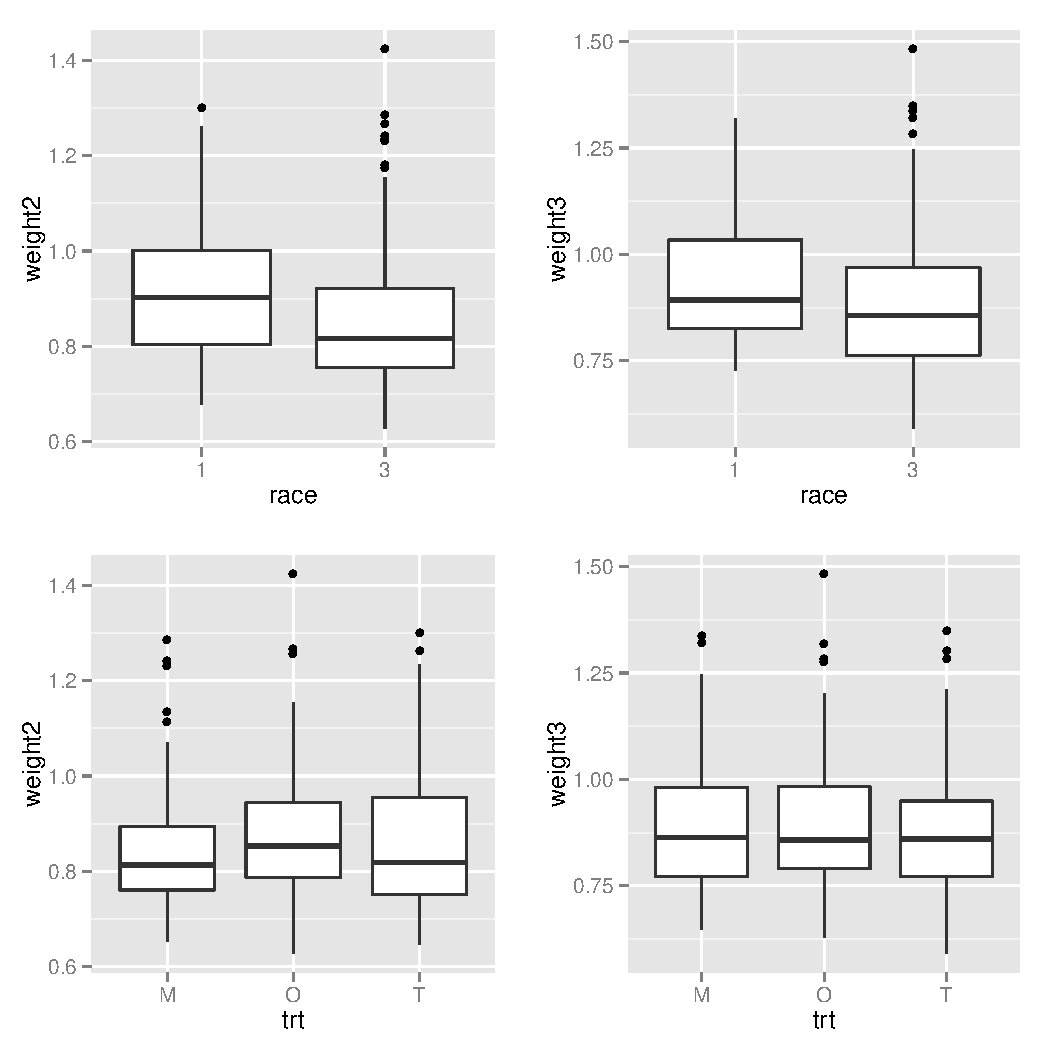
\includegraphics[scale = 0.8]{../tours/weight-plot}
\end{center}

Quantile regression models were fitted for responses \textit{weight2}
and \textit{weight3} together ($\bm Y_i = (Y_{i1}, Y_{i2})$) for
quantiles (10\%, 30\%, 50\%, 70\%, 90\%). Covariates are treatments
and races, and we assume their effects are additive. Treatment M and
Race 1 are baseline references. We fit 1,000 bootstraps to obtain the 
95\% confidence intervals. 

Estimates are presented in table \ref{tab:w2}. For \textit{weight2},
quantile estimates show there is no significant difference for three
treatment group through all the quantiles, because all 95 \%
confidence intervals include 0. However, when comparing weights from
two races, weights at 6th month from race 3 are generally lower than
ones from race 1. Estimates of race 3 effect to weights quantiles 10\%
up to 70\% are all significantly away from zero (negative). However,
for top weights of two races (90\% quantile), the difference is not
significant.

\begin{table}[ht]
  \renewcommand{\arraystretch}{1.3}
  \begin{center}
    \caption{Marginal quantile regression coefficients for
      Weight2}\label{tab:w2}
    \vspace{10pt}
    \begin{tabular}{rrrrr}
      \toprule
      & Intercept         & Trt.O                & Trt.T                & Race.3                \\ 
      \hline
      Weight2      &                   &                      &                      &                       \\ 
      $\tau$ = 0.1 & 0.80 (0.70, 0.86) & 0.01  ( -0.04, 0.07) & -0.01 ( -0.06, 0.06) & -0.13 ( -0.19, -0.04) \\ 
      $\tau$ = 0.3 & 0.83 (0.79, 0.92) & 0.04  ( -0.02, 0.07) & 0.02  ( -0.04, 0.05) & -0.07 ( -0.16, -0.03) \\ 
      $\tau$ = 0.5 & 0.85 (0.82, 0.98) & 0.05  ( -0.03, 0.09) & 0.04  ( -0.06, 0.07) & -0.03 ( -0.14, 0.00 ) \\ 
      $\tau$ = 0.7 & 0.95 (0.89, 1.03) & 0.03  ( -0.02, 0.10) & 0.02  ( -0.04, 0.08) & -0.04 ( -0.12, 0.00 ) \\ 
      $\tau$ = 0.9 & 0.98 (0.94, 1.11) & 0.07  ( -0.02, 0.14) & 0.06  ( -0.02, 0.14) & -0.01 ( -0.10, 0.05 ) \\
      Weight3      &                   &                      &                      &                       \\ 
      $\tau$ = 0.1 & 0.78 (0.38, 0.84) & -0.01 ( -0.07, 0.06) & -0.04 ( -0.10, 0.04) & -0.13 ( -0.18, -0.02) \\ 
      $\tau$ = 0.3 & 0.82 (0.78, 0.93) & 0.01  ( -0.04, 0.06) & -0.01 ( -0.07, 0.05) & -0.06 ( -0.16, -0.01) \\ 
      $\tau$ = 0.5 & 0.88 (0.84, 1.00) & 0.02  ( -0.06, 0.06) & 0.02  ( -0.08, 0.06) & -0.03 ( -0.13, 0.02 ) \\ 
      $\tau$ = 0.7 & 0.99 (0.92, 1.07) & 0.00  ( -0.05, 0.08) & -0.00 ( -0.07, 0.06) & -0.04 ( -0.12, 0.01 ) \\ 
      $\tau$ = 0.9 & 1.02 (0.98, 1.16) & 0.05  ( -0.06, 0.11) & 0.04  ( -0.05, 0.12) & 0.00  ( -0.10, 0.06 ) \\ 
      \bottomrule
    \end{tabular}
  \end{center}
\end{table}

For weights at 18th month (weight3), we have similar
conclusions. Confidence intervals of treatment effects on weight3 for
all quantiles (10\% up to 90\%) include zero. But after 18 months,
weights of patients from race 3 are significantly lower than ones from
race 1 only for lower quantiles (10\% to 30\%). They are not
significantly different for quantiles (50\% to 90\%).

\section{Identifiability}

First consider univariate case with two patterns. Suppose $y$ is
univariate and there are two patterns $R = 1$ and $R = 0$.

Before going forward to quantile regression, first we consider
identifiability problem in mean regression.

Consider a pattern mixture model:
\begin{align*}
  y | R = 1 & \sim N(\Delta + R_1 , \sigma_1) \\
  y | R = 0 & \sim N(\Delta + R_0, \sigma_0) \\
  \prob (R = 1) & = \pi \\
  E (y ) & = \theta
\end{align*}
Thus by iterated expectation, we have
\begin{align*}
  \theta = \Delta + R_1\pi + R_0(1-\pi) \\
  \Delta = \theta - \pi R_1 - (1 - \pi)R_0
\end{align*}
We can see $\Delta$ is deterministic by $\theta, R_1, R_0$. If plugged
in likelihood, we have
\begin{align*}
  y | R = 1 & \sim N(\theta + (1 - \pi)R_1 - (1 - \pi)R_0, \sigma_1) \\
  y | R = 0 & \sim N(\theta - \pi R_1 + \pi R_0, \sigma_0)
\end{align*}
Denote $\xi_1 = (\theta , R_1, R_0)$, and if $\xi_2 = (\theta, R_1+ 1,
R_0+1)$, both parameters lead to the same distribution of $\pr(y, R) =
\pr(y|R)\pr(R)$. Therefore, $\xi$ is not identifiable.  If we put
constraints on $R_1$ and $R_0$, for example $R_0 = -R_1$, then
\begin{align*}
  y | R = 1 & \sim N(\theta + 2(1 - \pi)R_1 , \sigma_1) \\
  y | R = 0 & \sim N(\theta - 2\pi R_1 , \sigma_0)
\end{align*}
thus it is identifiable. If $\xi_2 \neq \xi_1$ , then $\pr_2(y, R)
\neq \pr_1(y, R)$.

Secondly, we consider quantile regression for pattern mixture model:
\begin{align*}
  y | R = 1 & \sim N(\Delta + R_1 , \sigma_1) \\
  y | R = 0 & \sim N(\Delta + R_0, \sigma_0) \\
  \prob (R = 1) & = \pi \\
  \pr (y \leq \theta ) & = \tau
\end{align*}
where $\theta$ is the quantile estimate of interest and we does not
include covariates so far. We will show $\bm \xi = (\theta, R_1, R_0)
$ is not identifiable.

Again by iterated expectation, we have
\begin{align*}
  \tau = \pi \Phi \left( \frac{\theta - \Delta - R_1}{\sigma_1}
  \right) + (1 - \pi) \Phi \left( \frac{\theta - \Delta -
      R_0}{\sigma_0} \right)
\end{align*}
thus $\Delta$ is again deterministic by other parameters:
\begin{align*}
  \Delta = h(\theta, R_1, R_0, \sigma_1, \sigma_0 , \pi, \tau)
\end{align*}
To show $\bm \xi = (\theta, R_1, R_0, \sigma_1, \sigma_0)$ is not
identifiable, we need to find $\bm \xi^{'} \neq \bm \xi$, such that
$\pr(y|R) = \pr^{'}(y|R)$. If the last equation holds, then we must
have $\sigma_1^{'} = \sigma_1, \sigma_0^{'} = \sigma_0$, thus we still
need to find $\theta^{'} , R_1^{'}, R_0^{'}$ such that
\begin{align*}
  h(\bm \xi) + R_1 & = h(\bm \xi^{'}) + R_1^{'} \\
  h(\bm \xi) + R_0 & = h(\bm \xi^{'}) + R_0^{'}
\end{align*}
By substracting previous equations, we have $R_1^{'}- R_0^{'} = R_1-
R_0$, thus denote $R_1^{'} = R_1 + \delta$ and $R_0^{'} = R_0 +
\delta$, and let $\theta^{'} = \theta$ such that
\begin{align*}
  \Delta^{'} = h(\theta^{'}, R_1, R_0, \sigma_1, \sigma_0, \delta) =
  h(\bm \xi) - \delta = \Delta - \delta
\end{align*}
then the new parameter $\bm \xi^{'}$ yields the same distribution with
one from $\bm \xi$. Therefore $\bm \xi$ is not identifiable.

Instead, if we put constraint, for example $R_1 = -R_0$, then by
calculation, $\pr(y|R;\bm \xi) = \pr(y|R; \bm \xi^{'})$ yields $\bm
\xi = \bm \xi^{'}$.

Now consider the case with covariates. Suppose the model is
\begin{align*}
  y | R = 1, x & \sim N(\Delta + R_1 + \beta_{x1} x , \sigma_1) \\
  y | R = 0, x & \sim N(\Delta - R_1 + \beta_{x0} x, \sigma_0) \\
  \prob (R = 1) & = \pi \\
  \pr (y \leq \gamma_0 + \gamma_1 x ) & = \tau
\end{align*}
Still $\Delta$ can be determined by
\begin{align*}
  \Delta = h(x, \gamma_0, \gamma_1, R_1, \beta_{x1}, \beta_{x0},
  \sigma_1, \sigma_0, \pi , \tau)
\end{align*}
We want to show parameter $\bm \xi = (\gamma_0, \gamma_1, R_1,
\beta_{x1}, \beta_{x0}, \sigma_1, \sigma_0, \pi )$ is not identifiable
by finding $\bm \xi^{'} \neq \bm \xi$, but $\pr (y | R; \bm \xi) = \pr
(y | R; \bm \xi^{'})$. Still if the last equation holds, first we have
$\sigma_1^{'} = \sigma_1, \sigma_0^{'} = \sigma_0$, then to equate the
two means, we have
\begin{align*}
  \Delta + R_1 + \beta_{x1} x & = \Delta^{'} + R_1^{'} + \beta_{x1}^{'}x \\
  \Delta - R_1 + \beta_{x0} x & = \Delta^{'} - R_1^{'} +
  \beta_{x0}^{'}x
\end{align*}
By substracting the two equations, we have
\begin{align*}
  2R_1 + (\beta_{x1} - \beta_{x0}) x = 2R_1^{'} + (\beta_{x1}^{'} -
  \beta_{x0}^{'}) x
\end{align*}
which holds for all $x$. Thus $R_1 = R_1^{'}$ and $(\beta_{x1} -
\beta_{x0}) = (\beta_{x1}^{'} - \beta_{x0}^{'})$. Then let
\begin{align*}
  \beta_{x1}^{'} =  \beta_{x1} + \delta\\
  \beta_{x0}^{'} = \beta_{x0} + \delta
\end{align*}
and all the other parameters in $\bm \xi^{'}$ keep the same, we can
still have the same distribution of $y|R; \bm \xi$ but with different
$\bm \xi$. Therefore, $\bm \xi$ is not identifiable, especially for
$\beta_{x1} $ and $\beta_{x0}$. One solution is to restrict
$\beta_{x1} = - \beta_{x0}$ to make all the parameters identifiable.

Now consider the bivariate $(y_1, y_2)$ case, and we focus on the
identifiability issue especially on $y_2|y_1$. Suppose the model is
\begin{align*}
  y_2 | y_1, x, R = 1 \sim N(\Delta + R_1 + x\beta_{x1} + \beta_{11}y_1, \sigma_1) \\
  y_2 | y_1, x, R = 0 \sim N(\Delta - R_1 - x\beta_{x1} +
  \beta_{10}y_1, \sigma_0)
\end{align*}
Here $R$ stands for two different patterns, and missingness is not
considered.

we are wondering if $\beta_{11}$ and $\beta_{10}$ are identifiable,
say if there exists $\beta_{11}^{'}$ and $\beta_{10}^{'}$, such that
\begin{align*}
  \Delta + R_1 + x\beta_x + \beta_{11}y_1 = \Delta^{'} + R_1^{'} + x\beta_{x}^{'} + \beta_{11}^{'}y_1\\
  \Delta - R_1 - x\beta_x + \beta_{10}y_1 = \Delta^{'} - R_1^{'} -
  x\beta_{x}^{'} + \beta_{10}^{'}y_1
\end{align*}
still by substracting two equations, we have $R_1 = R_1^{'}$ and
$\beta_x = \beta_x^{'}$. Considering $\Delta$ is determined by
integrating out $y_1$, such that matching the two sides of the above
equation for coefficient of $y_1$, we must have $\beta_{11} =
\beta_{11}^{'}$ and $\beta_{10} = \beta_{10}^{'}$, therefore, $\bm
\xi$ is identifiable.

For identifiability issue in heterogeneous model described in section
\ref{sec:heter}, it is easy to show there is no trouble with 
heterogeneity parameters $\alpha$, analog to the linear model
case. For the other parameters, it can be found similar to the above
discussion.

\section{Quantiles for Contrasts}
We want to show quantiles for contrasts are deterministic if we model
the marginal quantiles simultaneously. For easiest case, (no mixture
model, only intercept):
\begin{align*}
  \tau & = \pr(y_1 \leq \theta_1)  \quad y_1\sim N(\Delta_1, \sigma_1^2) \\
  \tau & = \pr (y_2 \leq \theta_2) \quad y_2 |y_1 \sim N(\Delta_2 + \beta y_1, \sigma_2^2)
\end{align*}
Integrating out $y_1$ in conditional distribution $y_2|y_1$ , we have
\begin{align*}
  y_2 \sim N(\Delta_2 + \beta \Delta_1, \sigma_2^2 + \sigma_1^2 \beta^2)
\end{align*}
Thus, $\Delta_1$ and $\Delta_2$ can be solved by $\Delta_1 = \theta_1 - \sigma_{1}\Phi^{-1}(\tau)$ and $\Delta_2 =
\theta_2 - \beta \Delta_1 - \sqrt{\sigma_1^2\beta^2+\sigma_2^2}\Phi^{-1}(\tau)$.

So if we want to estimate quantiles for $y_2 - y_1$ too, such that:
\begin{align*}
  \tau = \pr (y_2 - y_1 \leq \theta)
\end{align*}
First we have
\begin{align*}
  Y_2 - y_1 |y_1 \sim N(\Delta_2 + (\beta- 1)y_1, \sigma_2^2)
\end{align*}
Integrating $y_1$ out, we have :
\begin{align*}
  y_2 - y_1 \sim N(\Delta_2 + (\beta-1)\Delta_1, \sigma_1^2(\beta-1)^2 + \sigma_2^2)
\end{align*}
Thus
\begin{align*}
  \theta & = \Delta_2 + (\beta-1)\Delta_1 + \sqrt{\sigma_1^2(\beta-1)^2+\sigma_2^2} \Phi^{-1}(\tau) \\
    & = \theta_2 - \theta_1 + \left( \sigma_1 + \sqrt{\sigma_1^2(\beta-1)^2+\sigma_2^2} -
    \sqrt{\sigma_1^2\beta^2+\sigma_2^2}\right) \Phi^{-1}(\tau)
\end{align*}
which is a functional of other parameters.

For the similar quantile regression with single covariates $x$,
suppose the model is :
\begin{align*}
  \tau &= \pr(y_1 \leq \theta_{01} + x\theta_{11} ), \quad Y_1 \sim N(\Delta_1, \sigma_1^2)\\
  \tau &= \pr (y_2 \leq \theta_{02} + x\theta_{12}) , \quad Y_2 | Y_1 \sim N(\Delta_2
  + \beta_yy_1, \sigma_2^2)
\end{align*}
similarly, we can solve $\Delta_2, \Delta_1$ by other parameters:
\begin{align*}
  \Delta_1 & = \theta_{01} + x\theta_{11} - \sigma_1\Phi^{-1}(\tau)\\
  \Delta_2 & = \theta_{02} + x\theta_{12} - \beta_y \Delta_1 - \sqrt{\sigma_2^2 +
    \beta_y^2\sigma_1^2} \Phi^{-1}(\tau)
\end{align*}
Now what if we want to estimate quantile regression for contrast $Y_2 -
Y_1$:
\begin{align*}
  \tau = \pr (Y_2 - Y_1 \leq \theta_0 + x\theta_1)
\end{align*}
we will have
\begin{align*}
  (\theta_{02} - \theta_0) + x(\theta_{12} - \theta_1) = \theta_{01} + x\theta_{11} +
  \left( \sqrt{\sigma_2^2 + \beta_y^2\sigma_1^2} - \sqrt{\sigma_2^2 + (\beta_y-1)^2\sigma_1^2} -\sigma_1 \right)
  \Phi^{-1}(\tau)
\end{align*}
Since it holds for all $x$, then :
\begin{align*}
  \theta_1 &= \theta_{12} - \theta_{11} \\
  \theta_0 & = \theta_{02} - \theta_{01} - \left( \sqrt{\sigma_2^2 + \beta_y^2\sigma_1^2} -
    \sqrt{\sigma_2^2 + (\beta_y-1)^2\sigma_1^2} -\sigma_1 \right) \Phi^{-1}(\tau)
\end{align*}
  
For mixture normal margins, similarly quantile regressions for
contrasts are determined by parameters in original models, since the
distribution of contrasts is determined by joint
distribution. Simultaneously modeling these parameters would become
problematic, but using plug-in estimators could be one option.

\end{document}
